\chapter{实验}
\label{chap4}

\section{实验设计}

本文中使用sumo作为仿真实验工具,生成模拟道路和信号灯,并且在地图上随机生成车辆获取车辆的轨迹信息来进行仿真试验。参数的设置为每段路的长度为1500m,车辆限速初始为90km\textbackslash h,实验过程中会视情况调整,一个交通信号灯的周期为140s,其中每个方向直行放行40s之后左转放行30s,右转方向为全时绿灯的状态。

\begin{figure}[H] 
  \centering
  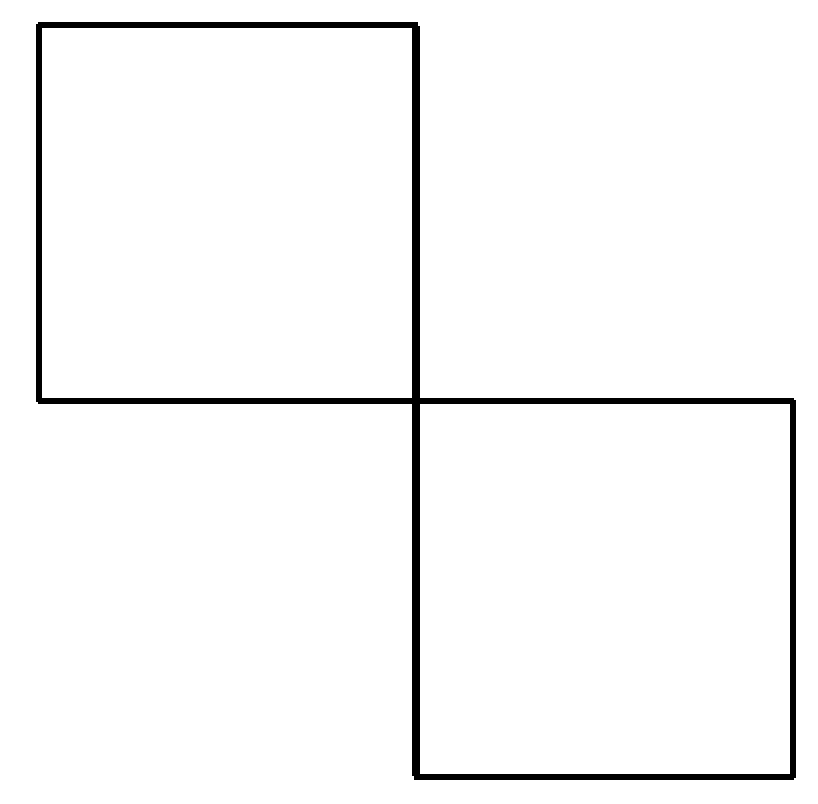
\includegraphics[width=2.5in]{simulation}
  \caption{地图}
  \label{fig:4.1}
\end{figure}

为了让轨迹数据能够集中通过十字路口,主要地图设计成如图\ref{fig:4.1},为一个"8"字形地图,使得随机的车辆能够在地图中随意行驶并且集中地通过中心的路口。

\begin{figure}[H] 
  \centering
  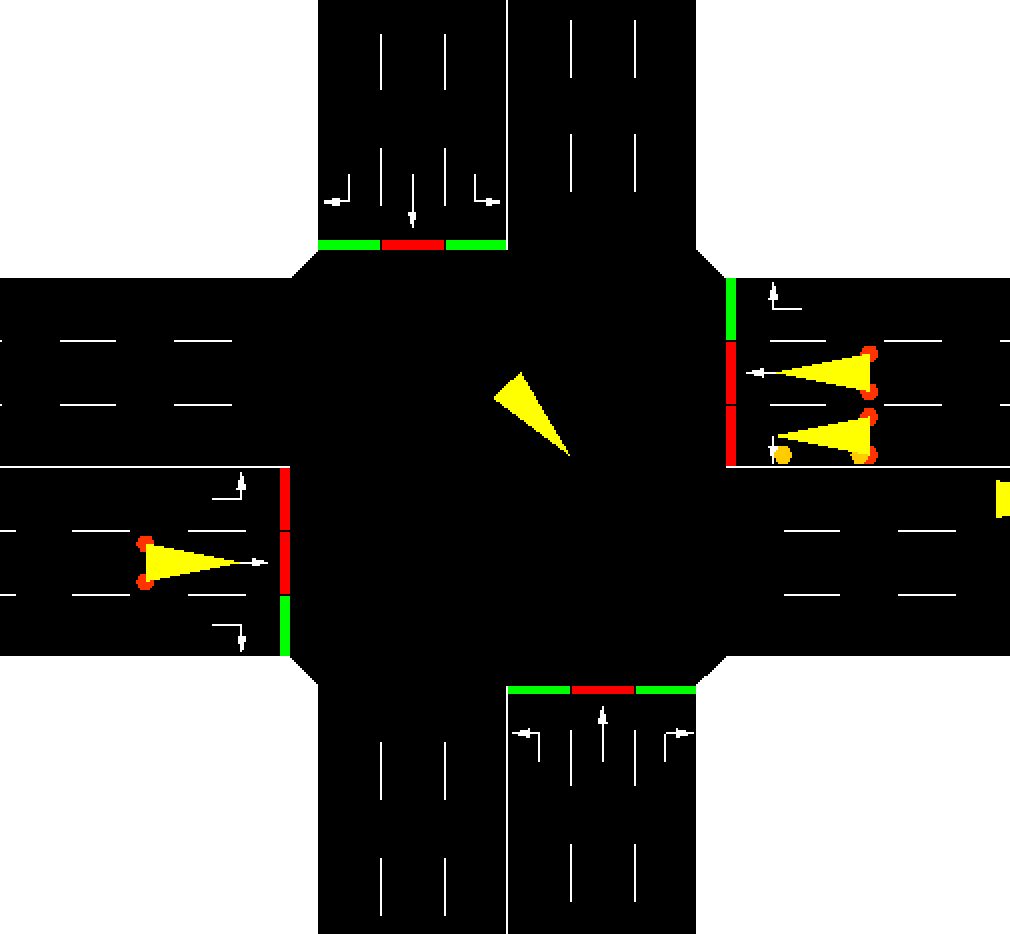
\includegraphics[width=3in]{cross}
  \caption{路口放大}
  \label{fig:4.2}
\end{figure}

模拟过程可以通过sumo-gui直观地看到,可以观察每辆车的具体行驶轨迹,路口模拟效果如图\ref{fig:4.2},可以清晰地看到每辆车和红绿灯的状态。

\section{实验结果分析}

\subsection{对比Bayes和最小二乘法}
从图\ref{fig:4.8}中我们可以看到,Bayes方法在数据量较少的时候更加稳定,准确度也比最小二乘法更高,最小二乘法等价于最大似然估计,在数据量小的时候会出现过拟合的现象,但是随着数据量逐渐增加准确度会超过Bayes方法,所以我们会在数据量较少(少于14组时)使用Bayes方法拟合,在数据量较多的时候使用最小二乘法进行更精确的估计,将两种算法结合到一起。

\begin{figure}[H] 
  \centering
  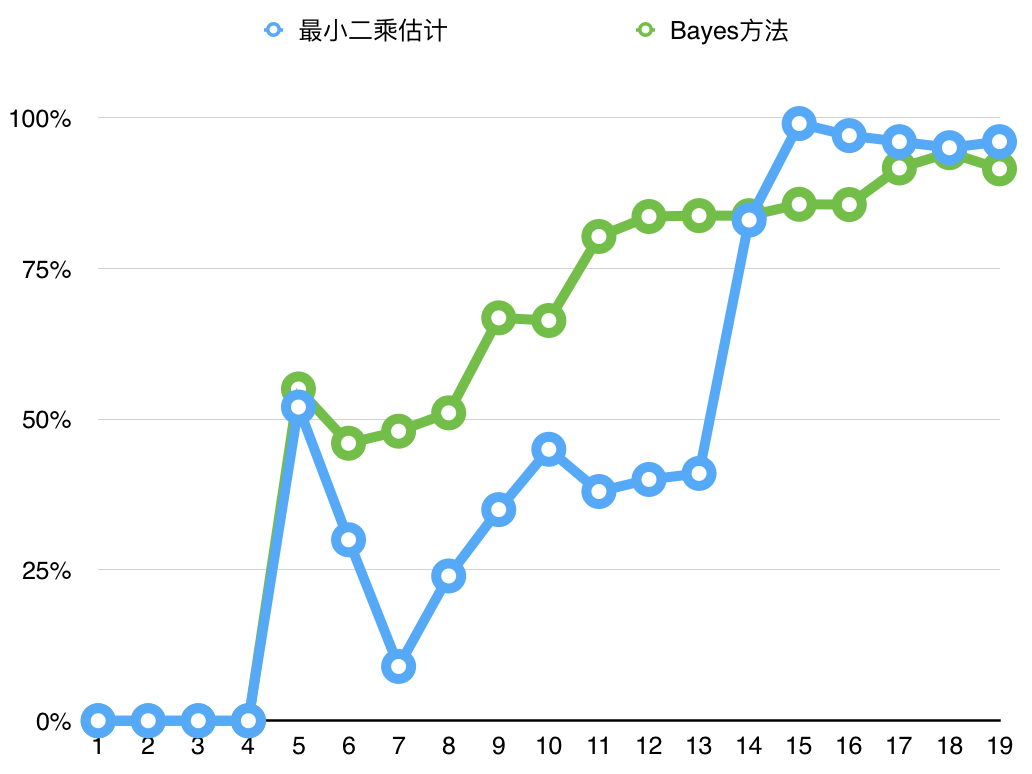
\includegraphics[width=3.5in]{bayes}
  \caption{两种方法对比}
  \label{fig:4.8}
\end{figure}

\subsection{单方向}
利用sumo中的轨迹GPS数据,选取单方向统计5分钟内的轨迹作为输入,之后将估计的两段路的路况与计算出的实际路况进行比对计算出准确率,直行方向和右转方向准确度与轨迹条数的关系见图\ref{fig:4.3}和图\ref{fig:4.4}。

\begin{figure}[H] 
  \centering
  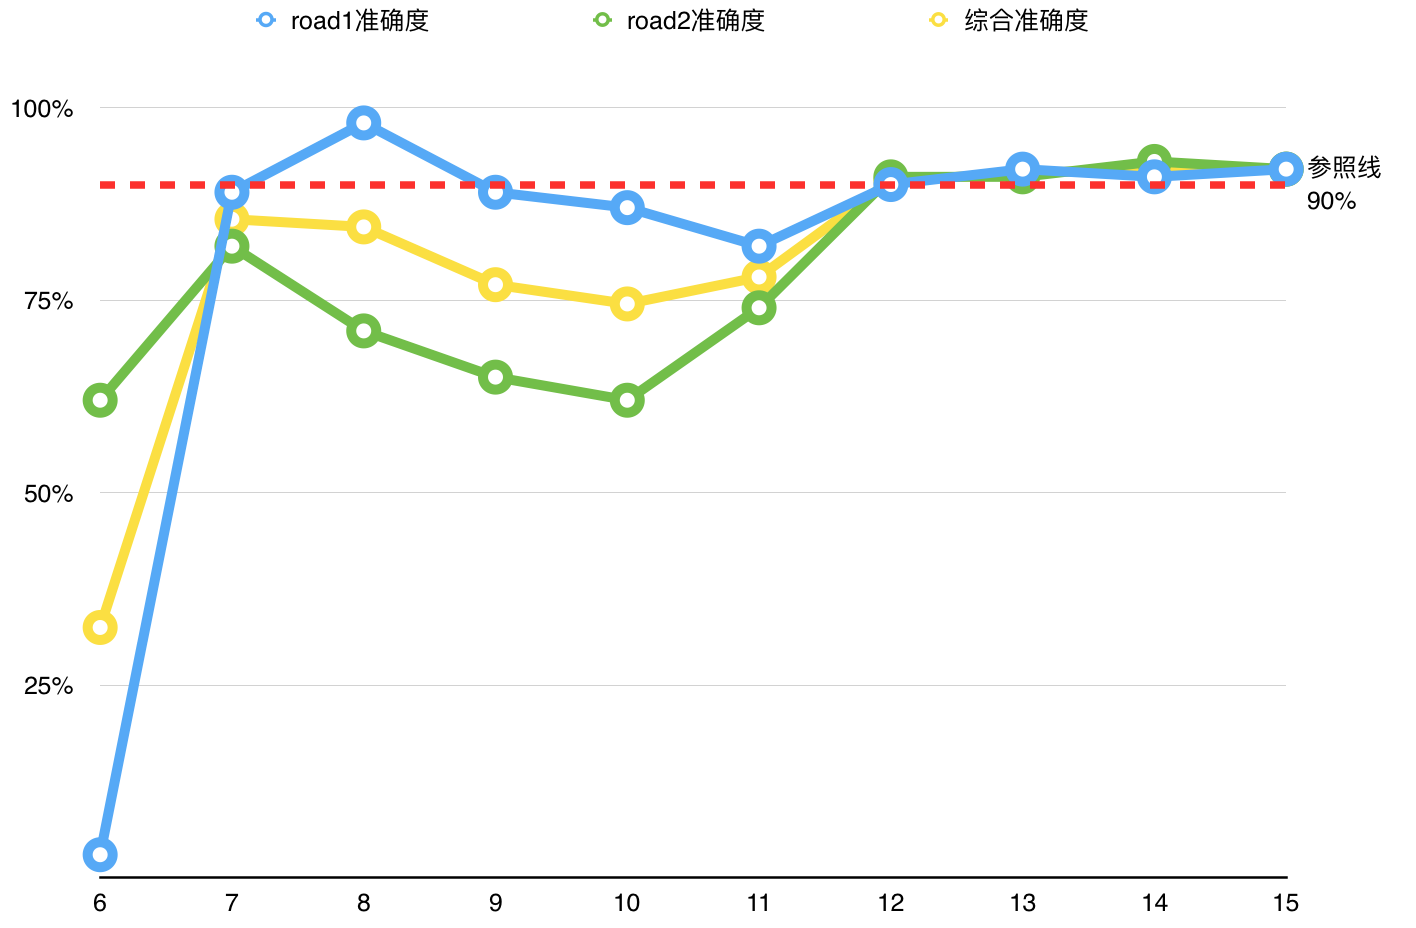
\includegraphics[width=3.5in]{result1}
  \caption{直行方向准确度}
  \label{fig:4.3}
\end{figure}

\begin{figure}[H] 
  \centering
  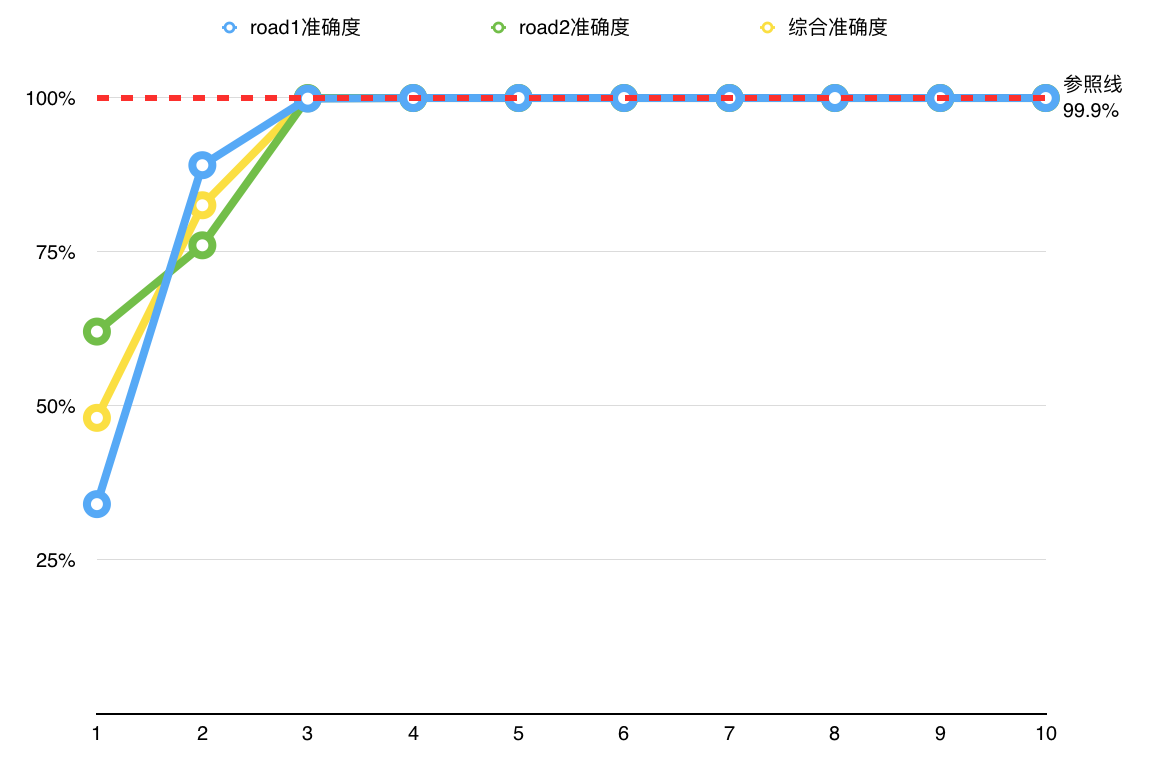
\includegraphics[width=3.5in]{result_right_turn}
  \caption{右转方向准确度}
  \label{fig:4.4}
\end{figure}

从图中我们可以看到直行方向大概需要12条轨迹数据来达到总体90\%的准确率,7条轨迹到11条轨迹之间的结果存在波动,分析数据得出出现波动的原因是其中中间几组数据的信号灯等待时间较长,导致算法回归时直线出现了便宜,数据量再增加直到12条之后,个别数据的偏移不会对总体数据造成很大的影响,左转方向与直行方向的情况基本相同。而右转方向因为无需等待交通信号灯,所以转向延迟比较稳定,采用我们的算法,只需要3条轨迹信息就可以到达99.9\%的正确率。

\subsection{与原有的平滑算法的对比}
当单方向两段路路况存在较大差异时,即一段路堵塞而另一段正常行驶,给出方向有15组GPS轨迹信息,分别使用平滑和线性回归两种算法计算两段路的路况,得出结果如图\ref{fig:4.7}
\begin{figure}[H] 
  \centering
  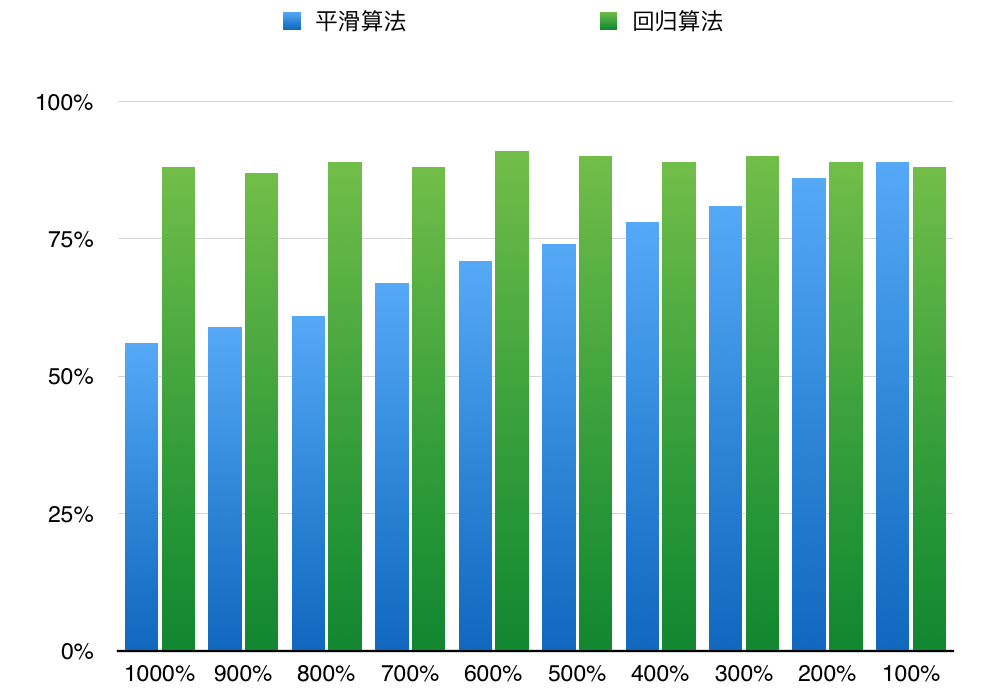
\includegraphics[width=3in]{difference}
  \caption{路况差异较大时两种算法的对比}
  \label{fig:4.7}
\end{figure}
图\ref{fig:4.7}中横坐标为一条轨迹经过两段路段平均速度的比例,纵坐标为路况计算的准确率。实验中我们通过限制一段路的最高速度使得两个路段的畅通程度产生差异。例如横坐标1000\%的点,我们取一段路最高限速为25km\textbackslash h,另一段路最高限速为2.5km\textbackslash h,给出15组车辆轨迹数据,分别用两种方法算出两段路的路况与实际值做对比。我们可以看出,当两个方向的平均速度相差1000\%时,回归算法对比平滑算法优势明显,随着两段路速度差异的变小,算法的准确率差距也逐渐缩小,最后两段路况基本相同时,两种算法的准确率都稳定到90\%左右。

\subsection{三方向混合}
对于经过同一路段的三个方向轨迹信息进行混合,先拿出右转方向的轨迹信息计算出该路段的路况,再将其应用到直行和左转方向的路况计算中,计算下一路段的路况,得出结果如图\ref{fig:4.5}。

\begin{figure}[H] 
  \centering
  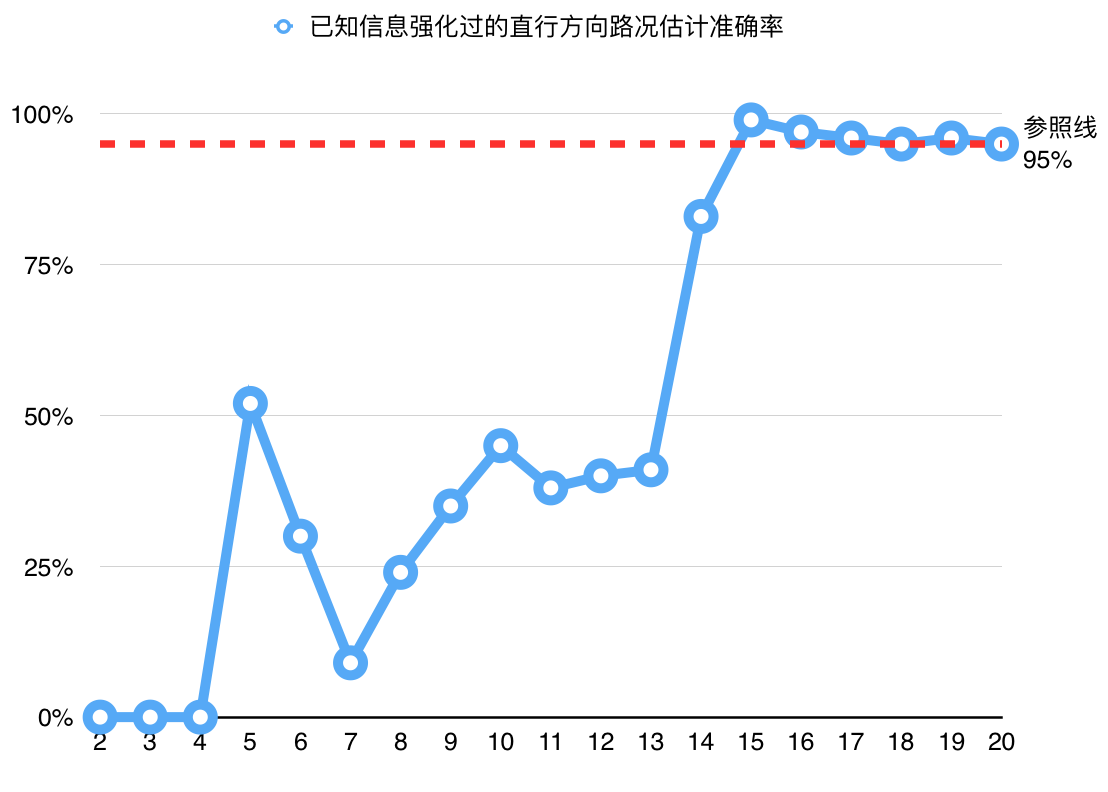
\includegraphics[width=3.5in]{result2}
  \caption{三方向混合准确度}
  \label{fig:4.5}
\end{figure}

从图中我们可以发现,直行方向此时需要15条轨迹数据来达到稳定的准确率,比之前直接对该方向轨迹进行回归的12条还多出三条,这种情况出现的原因是确定前一段路况之后,线性回归又三维降低为二维,但是常数项也就是路口延迟的波动对于我回归的影响会变得更严重,但是达到稳定状态后,我们可以得到比前面更优的结果,准确率为95\%以上,所以我们决定综合使用这两种方法,在轨迹数为14条及以下时直接计算该方向路况,在15条及以上时使用右转方向的既得信息对回归降低维度,得到更精准的结果。

\subsection{全方向混合}
考虑到相对方向的路口信号灯等待和通行周期相同,如果我们得到一个方向的转向延迟,我们就可以把转向延迟应用到其对应方向的计算中,使准确率得到提高。结果如图\ref{fig:4.6}。

\begin{figure}[H] 
  \centering
  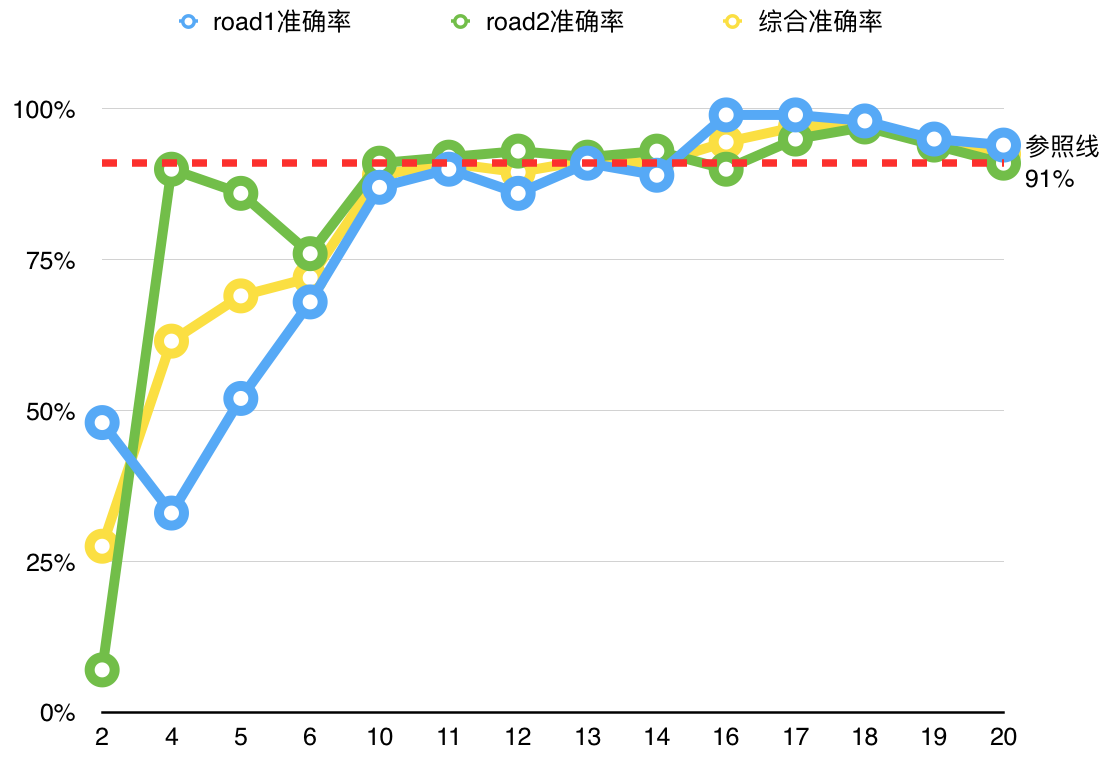
\includegraphics[width=3.5in]{result3}
  \caption{全方向混合准确度}
  \label{fig:4.6}
\end{figure}

从图中我们可以看出得到对应方向的转向延迟信息后,该方向只需要10条轨迹就可以计算出准确率为91\%左右的路况信息,对应方向提供的转向延迟信息可以帮助筛选该方向的数据,规避掉路口信号灯等待时间过长的轨迹信息带来的影响,所以可以使得路况计算所需的轨迹数量减少。

\section{小结}
通过仿真数据的验证,说明了我们的模型对于轨迹数量较多的稀疏数据能够有很高的路况估计准确率。在我们的模型中,对于一个十字路口,最理想的情况是有四个右转方向各三组以上的轨迹数据,这样就能精确地得到8个方向的路况,共需12组轨迹,得到99\%准确率的路况信息。最不理想的情况是没有右转方向的轨迹,这种情况下,我们结合路口对应方向的路况信息,每组对应方向至少需要12+10=22组轨迹信息来得到准确率高于90\%的路况信息,这样加起来就需要至少22*2=44组轨迹信息来得到8个方向的路况。